\chapter{Web Performance Metrics}
\label{chap:metrics}
Before any measurement or even improvement regarding a website's performance can be made, it's important to understand what actually are the reasons for the delay until a user can see the rendered webpage in her browser. 
\begin{figure}[h]
	\centering
      		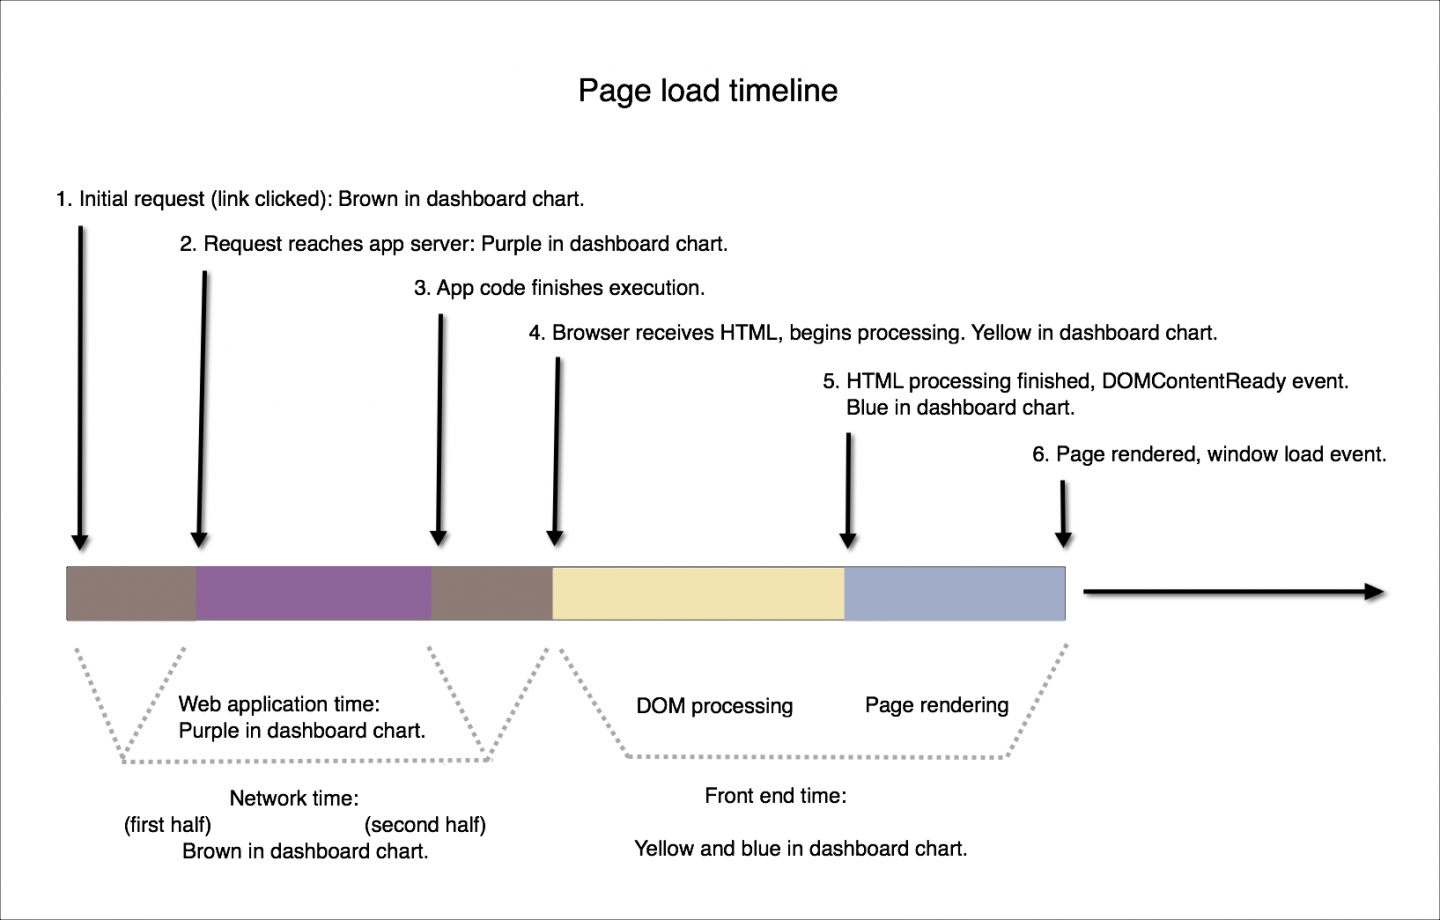
\includegraphics[width=0.9\textwidth]{imgs/timeline}
  	\caption{Timeline of a page load \cite{NewRelic_Load}}
\end{figure}
Since a website is not like an executable started at the computer of a client, there are several indicators affecting the overall performance of a website at which I want to look at in more detail now.  

\section{Latency}
Latency basically is the time it takes a message to travel from it's point of origin to the destination. Although this sounds very simple, it's clear that not every source in the network is directly connected to a destination point. The global network infrastructure is much more complex and therefore several components contribute to the overall latency. In essence latency can be grouped into:
\begin{itemize}
	\item{Propagation delay}
	\item{Transmission delay}
	\item{Processing delay}
	\item{Queuing delay}
\end{itemize}

\textbf{Propagation delay} is the time required for a network packet to travel from sender to receiver. It simply can be computed as a function of distance over speed and is heavily based on the speed of light, the maximum speed at which information can travel. Fortunately the speed of light is extremely fast and even including a small loss of speed due to refraction of the medium through which the message travels it only takes a few hundred milliseconds to cross the distance between two continents. There have been a lot of improvements regarding the medium connecting network components and with fiber-optic cables a speed of approximately 200.000m/s can be achieved nowadays \cite{Grigorik_2013}.

\begin{table}[h]
\begin{center}
\begin{tabular}{| c | c | c | c |}
    \hline
    Route & Distance & Time (vaacum) & Time (fiber) \\ \hline
    New York to San Francisco & 4.148km & 14ms & 21ms  \\ \hline
    New York to London & 5585km & 19ms & 28ms \\ \hline
    New York to Sydney & 15993km & 53ms & 80ms \\ \hline 
     Equatorial circumference & 40075km & 133.7ms & 200ms \\
    \hline
\end{tabular}
\caption{Examples for propagation delays \cite{Grigorik_2013}}
\end{center}
\end{table}

\textbf{Transmission delay} is the time it takes to put the packet to be sent onto the data link \cite{Grigorik_2013}. The bytes to be sent over the network are not automatically on the link and therefore there must be this delay. Due to the small size of request and response packets as they are used for websites, this amount of time usually stays within a few milliseconds. It can also be described as a function of packet length divided by data rate of the link.

The latencies presented the table above assume a direct connection between two locations. In practice this does not hold since a packet gets handled by several intermediate routers until it reaches the destination. Each router must accept the incoming packet first, look at the header information of it and decide where to send the packet next. The time required for these operations is called \textbf{Processing delay}.  This delay can vary from packet to packet and strongly depends on the number of hops a packet does on it's way \cite{Killelea_2002}. Nearly all of the operations are done in the hardware and cost less time \cite{Grigorik_2013}.

Due to everyday's enormous amount of traffic the network can be unpredictable under some circumstances. If the traffic load on routers is high some packets have to be put into an incoming buffer and will be queued before they can be processed. This is known as \textbf{Queuing delay} and can add some additional time to overall latency. The concerned routers on the way usually vary in latency and bandwidth as well as the traffic along the path which makes it difficult to predict occurrence of queuing.   

The sum of these delays results in the total network latency and under normal circumstances does not exceed about 300ms, even when crossing oceans and continents \cite{Grigorik_2013}. Although these delays don't seem to introduce any kind of problem, especially when we consider such extraordinarily large distances like in the example, the parameter latency is critical and can introduce a performance bottleneck. This will get clearer when looking at the involved protocols by a request.

\section{Throughput}
Throughput is the number of items processed per unit time, such as operations per minute or instructions per second. When talking about network connections the term Bandwidth is usually used instead, which is equal to the throughput in bits per second. 
Regarding bandwidth there hast be differentiated between the core network and the edge points. 

\textbf{Bandwidth in core networks} is the bit rate per seconds for links across long distances, like subsea connections between continents. Different cable mediums have been researched over years whereby with nowadays capabilities of fiber-optic connections, amazing rates of 70Tb/s for a single fiber-optic link could be reached.   

On the edges of the network things look completely different. \textbf{Bandwidth at edge points} is the data rate we know from our ISP and depends heavily at the technology used. No matter whether it is dial-up, DSL or fiber-optic to the home these numbers are very small compared to the core network bandwidth  \cite{Grigorik_2013}.

Bandwidth is not directly connected to Latency, which means that a low latency not necessarily implicates high bandwidth of the data link. However if we take the bandwidth at the network edge, an increase of maximum throughput often leads to lower latency since more packets can be processed in the same time and collisions and congestion will more likely be avoided. If the problem occurs at some intermediate hops on the path, higher bandwidth does not have any positive effect on latency \cite{Killelea_2002}.

\section{Utilization and Efficiency}
These two performance parameters give a more general indicator of the system's components performance. \textbf{Utilization} is the fraction of capacity of a component used \cite{Killelea_2002}. This gives a good hint how busy a server component currently is and how much load it can handle by operating still normal. There are a lot of common utilization performance metrics which can be measured. The most popular ones are
\begin{itemize}
	\item{CPU}
	\item{Disk}
	\item{Memory}
\end{itemize} 

Although these metrics are not directly connected to the performance a user experiences when she waits for a web page to be visible in the browser, it helps to check whether infrastructure components operate as expected. The reason for bad performance is not always based on poor latency or throughput, sometimes whole components does not scale as desired and this can have negative impact on what happens on the server side.

\textbf{Efficiency} is defined as throughput divided by utilization. Efficiency cannot be measured but can reveal how much components can withstand. This metric can further have some influence in economic decisions when deciding about buying resources. In this case it is more likely known as cost-effectiveness. \cite{Killelea_2002}
   
\section{Processing Time on Server}
This is the time between the arrival of the request on the server and the point where the server starts to send the response. For the performance of a web application it is an important metric as it gives information how fast the server fetches and builds the web resource requested. Since modern websites don't contain only pure HTML code usually much more work has to be done to generate the outgoing response file. This includes algorithms to be executed, working with databases in the backend, pre-processing CSS and Javascript extensible languages, loading of images, generating HTML and so forth. Interactive web applications which work with bigger datasets can lack of performance pretty fast if you don't pay attention on using appropriate software technologies or doing cost-intensive work to fulfil interactive tasks of a user. 

\section{Browser Processing}

When the first bytes have arrived at the client it's time for the browser to start it's work. Obviously it is important for good user experience that the time span between a request and the arrival of the first byte should be as minimal as possible because during this time nothing can happen inside the browser. Similar to the networking and processing time there is potential to save time and improve user experience when making the website visible. 

\subsection{DOM Processing}
The first step the browser has to do is to identify the fetched resource from the server, where in it's simplest form it is HTML content. The received characters are disassembled into tokens and the DOM (Document Object Model) is constructed. The DOM is required to render any element on the screen and can be blocked by some other resources and therefore delayed. The same happens with CSS applied on HTML elements. For this purpose a so called CSSOM (CSS Object Model) gets constructed and afterwards combined with the DOM to a render tree ready for painting. Due to the reason that a website is effectively unusable without any style, CSS is basically treated as a render blocking resource and interrupts processing of other content. Another blocking resource is Javascript no matter if placed inline or within an external file. DOM construction will be interrupted if Javascript has to be executed. Processing the final DOM for first page view early shortens the time until elements appear on the screen and therefore this time point is a crucial one regarding any performance optimizations during web development. \cite{GoogleDev} 

\subsection{Page Rendering}
After the DOM and CSSOM have been constructed and composed to the render tree the elements can be painted onto the screen. Although much of the work is done automatically by the browser, there are some performance tweaks possible to significantly improve user experience. As metric which can be directly measured it is usually referred to the final onLoad-Event indicating the completeness of a page load when every element of the webpage is visible on the screen. However, most often it is more important to improve the visual appearing of single elements like text, images, multi-media content etc. There is a huge difference for the user whether one essential page element is visible after 0.3 seconds and the following after 0.6 seconds or both elements appear after 0.6 seconds. Page rendering is an important metric but has to be observed differently since here perceived experience is critical. 